\documentclass{article}
\usepackage[english]{babel}
\usepackage[utf8x]{inputenc}
\usepackage{amsmath}
\usepackage{graphicx}
\usepackage[colorinlistoftodos]{todonotes}
\usepackage{enumitem}
\usepackage{listings}
\usepackage{filecontents}
\usepackage{verbatim}
\usepackage{eurosym}
\usepackage{setspace}
\usepackage{natbib}
\usepackage[export]{adjustbox}
\usepackage{xcolor}
\usepackage{minted}
\usepackage{algorithm}
\usepackage[noend]{algpseudocode}
\usepackage{amssymb}
\usepackage{float}
\usepackage{subfig}
\usepackage{tocloft}
\usepackage{multicol}
% \usepackage[left=2.60cm, right=2.60cm, top=3.00cm, bottom=3.00cm]{geometry}
\usepackage{titlesec}

\usepackage{caption}


\titleformat*{\section}{\Large\bfseries}
\titleformat*{\subsection}{\large\bfseries}

\setlength{\columnsep}{15px}

\title{
  \textbf{\HUGE Aprendizaje Automático} \\
  \large Memoria de Prácticas 2
}
\author{\\\\Rafael Sanjuan Aguilera}
\date{Segundo Cuatrimestre, 2019}

\newcommand{\HRule}{\rule{\linewidth}{0.5mm}}

 
\definecolor{codegreen}{rgb}{0,0.6,0}
\definecolor{codegray}{rgb}{0.5,0.5,0.5}
\definecolor{codepurple}{rgb}{0.58,0,0.82}
\definecolor{backcolour}{HTML}{F8F8F8}
\definecolor{LightGray}{gray}{1}

\setminted[python]{
    framesep=2mm, 
    baselinestretch=1.2, 
    bgcolor=backcolour,
    fontsize=\footnotesize,
    linenos
}
 

\lstdefinestyle{mystyle}{
    backgroundcolor=\color{backcolour},   
    commentstyle=\color{codegreen},
    keywordstyle=\color{magenta},
    numberstyle=\tiny\color{codegray},
    stringstyle=\color{codepurple},
    basicstyle=\footnotesize,
    breakatwhitespace=false,         
    breaklines=true,                 
    captionpos=b,                    
    keepspaces=true,                 
    numbers=left,                    
    numbersep=5pt,                  
    showspaces=false,                
    showstringspaces=false,
    showtabs=false,                  
    tabsize=2
}

\lstset{style=mystyle}

\begin{document}

%----------------------------------------------------------------------------------------
%   TITLE PAGE
%----------------------------------------------------------------------------------------

\begin{titlepage}
\begin{center}

\textsc{\LARGE University of Granada}\\[1.5cm] % University name


\includegraphics[width=100px]{figures/ugrlogo.png}


\vfill
\HRule \\[0.4cm]
{\huge \bfseries Fitting Lineal Models}\\[0.4cm]
\textsc{\Large Machine Learning. Assignment 3}\\[0.5cm]
\HRule \\[1.5cm]
 

\begin{center}
    \textsc{RAFAEL SANJUAN AGUILERA} \\
\end{center}

\vfill
{\large March, 2019}\\[4cm] % Date

\vfill
\end{center}

\end{titlepage}

\newpage
\tableofcontents





~\\
~\\
~\\
\newpage

\pagenumbering{arabic}


%----------------------------------------------------------------------------------------
%   EJERCICIO 1
%----------------------------------------------------------------------------------------
% \section{Introduction}\normalsize
% \setcounter{section}{1}
% \doublespacing
% \singlespacing

% Este ejercicio se centra en el ajuste de un modelo lineal a conjuntos de datos dadas con el objetivo de obtener el mejor predictor posible. En todos los casos los pasos a desarrollar serán aquellos que nos conduzcan al ajuste y selección del mejor modelo y a la estimación del error $E_{out}$ del modelo final. Cómo mínimo se habrán de analizar y comentar los siguientes pasos sobre un problema de clasificación y otro de regresión:


% \newpage

% \begin{multicols}{2}
\begin{center}
    \textit{\textbf{Abstract}}
\end{center}

As an assignment for our Machine Learning module in Computer Engineering, we study two data sets with the objective of applying both theory and practice learnt in the module. With the imposed restriction of only using linear models, we take a look at a classification and a linear regression problem and discuss data processing, possible hypothesis sets, out of sample performance evaluation methodology and the effects in our results. We implement using ML two models, one of them able to classify hand-written digits with very good accuracy and the other is able to predict the noise of produced by the wind hitting an air vehicle.

\section{Classification. Hand-written numbers dataset.}

\subsection{Understanding the problem}

The problem at hand consists in the automatic classification of digits, more precisely in low resolution, square shaped, 2D images. 


For this task we are using a notably famous data set called \textit{Optical Recognition of Handwritten Digits Data Set}. This data is free and publicly available at the UCI website. \cite{Dua:2019}


\begin{figure}[H]
\centering
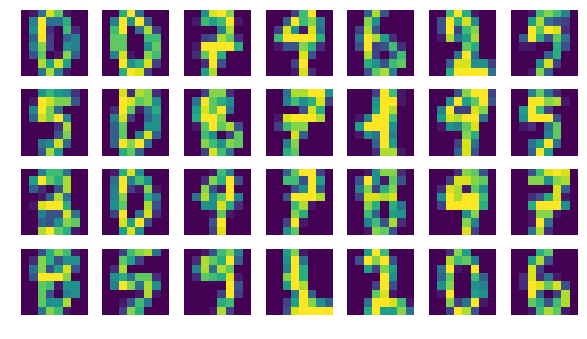
\includegraphics[width=240px]{figures/fig01}
\label{fig:Dataset visualization}
\caption{\footnotesize Visualisation of a small subset of trainig data.}
\end{figure}

Each input data element $x$ from the dataset $\mathcal{D}$ is a 64-dimensional vector. This vectors originate from a reshaped 8x8 matrix where each element is the result of the downsampling of a 32x32 bitmap into non-overlapping blocks of 4x4 and the numbers of pixels are counted for each block. This means each value of the vector is in the range [0, 16], the authors considered this gave invariance to small distortions while reducing dimensionality.

Is note-wordy to point out the data set comes already split in two files for training and testing with ".tra" and "tes" extensions respectably.

% From a total of 43 people, 30 contributed to the training set and different 13 to the test set. 32x32 bitmaps are divided into nonoverlapping blocks of 4x4 and the number of on pixels are counted in each block. This generates an input matrix of 8x8 where each element is an integer in the range 0..16. This reduces dimensionality and gives invariance to small distortions. 

% El problema consiste en la clasificación automática de dígitos, más concretamente en imágenes 2D cuadradas de baja resolución de la escritura a mano de estos dígitos.


% Para abordar este problema disponemos con una base de datos de dígitos compuesta de 6... vectores ...




\subsection{Data preprocessing} 
% $\to$ eliminar datos sin variabilidad, reducción/aumento de dimensionalidad, normalización de datos,…
As we commented in \S1.1 each parameter, block, in a data point $x$ is always in the same [0,16] range, thus, even though normalising the data is a big standard we don't deem it necessary.

Intuition leads us to hipotesize that some blocks of the bitmap will be very underused if relevant at all. Even if we consider the dimensionality of our data handleable with today's tools, we will experiment with dimensionality reduction to see the effects in performance.

For reducing the dimensionality of the input data we have used the technique Principal Component Analysis, PCA, the main reason of his usage is his general good behaviour and popularity of his application for this kind of problems.

PCA aims to find the dimensions of the dataset holding the most relevant information, most variance, and reducing the dimensionality by combining less relevant characteristics.


\subsubsection{Processing with PCA}
\begin{minted}{python}
 from sklearn.decomposition import PCA
 X_pca = np.copy(X_train)

 pca = PCA(n_components=0.99)
 X_pca = pca.fit_transform(X_pca) # , y_train
 print(X_pca.shape)
\end{minted}

\begin{minted}{python}[bgcolor=codepurple, linenos=False]
>>> (3823, 41)
\end{minted}

After applying PCA with a very high 99\% variance threshold we are surprised to get a heavily reduced dataset, only 41 elements, getting rid of near one third of the pixels in the bitmap.

\subsubsection{Visualising variance}
\begin{figure}[H]
    \centering
    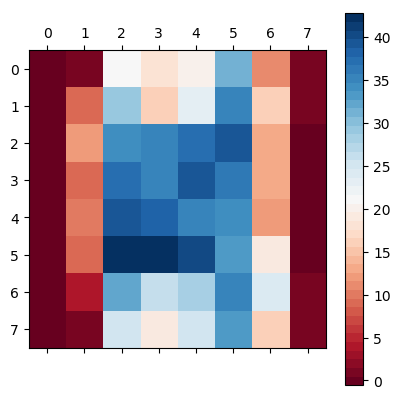
\includegraphics[width=140px]{figures/fig02.png}
    \caption{Pixel variance of the training dataset visualised as a heatmap.}
    \label{fig:variance-heatmap}
\end{figure}

Observing the figure 2, we can conclude that both first and last colunms of the dataset 2D images are less relevant data when discriminating the digits. This shouldn't come as any surprise as most people write numbers with bigger height than width, and so this gets reflected in the training data.

\subsection{Hypotesis set selection}
% $\to$ combinaciones lineales/cuadráticas/etc. de los valores observados
Although extracting higher abstraction descriptions of our input signal is a very powerful tool for making predictions in images, our input data is way smaller in dimension than most of the images that get handled this way. Many authors like Abu-Mostafa \cite{Abu-Mostafa:2012:LD:2207825} have extracted characteristics like symmetry or mean intensity for working with digit classification. Even if this is indeed a good approach, finding this higher level characteristics is not trivial, it's as difficult as finding a good heuristic for the problem at hand.

We have also seen in previous assignments that the aforementioned two characteristics in digit classification can both work wonderfully, for discriminating ones from fives, or terribly, for digits four and eight comparison.

Thus, we set on not making transformations outside of preprocessing in the input data.


\subsection{Testing methodology}
% $\to$ ¿uso de cross-validation?
In order to prevent bias in the training-test split we will use a very common testing split called k-fold cross-validation \cite{edsjsr.298480919740101}. This will mean splitting the data in k different splits and using k-1 of them for training and the left out fragment for validating the hypothesis obtained with the training data. We will also make sure to keep the ratio of appearance from each class in training and validation.



% Acc is an important metric because it reflects how the rate of success of our classifier, Sen tells us information about how likely we are to correctly identify each digit against the rest and Spe gives u 

% To evaluate the performance of the different models 3
% metrics per class were taken into account: Sensitivity (Sen),
% Specificity (Spe), and Accuracy (Acc). Sen refers to the true
% positive rate, measuring the proportion of actual positives
% which are correctly identified as such. Spe is the true negative
% rate and gives the proportion of negatives which are correctly
% identified as such. Acc is defined as the total number of
% true and false positives divided by the total number of cases
% examined (true positives, false positives, true negatives, and
% false negatives). These metrics are computed for each class
% independently.

After fixing our final model adjusting the hyperparameters to get the best performance inside our training data set, we will evaluate our classifier with the previously stored test data split.


\subsection{Regularization}
We will now talk about applying regularisation to our hypothesis set.

It is our main interest when adjusting any model to get the best performance out of sample, $E_{out}$, meaning our model generalises well. 

In seeking this good generalisation we try to prevent adjusting to the error in our input data, overfitting.
Regularising takes part in almost any machine learning problem, is our tool to prevent overfitting by lowering the variance of the model with minimal bias penalisation.

In practice all the linear models used for this experiment have a $C$ parameter in the \textit{sklearn} library set to a default $1.0$.

\[C=\frac{1}{\lambda}\]

As his description says in the documentation is the inverse of the regularisation strength. We will set this parameter to soften the adjust of the model to the training data using cross-validation tests in sample as descrived in \S 1.4


\subsection{Models used and hyperparamethers}
% Our simplest algorithm, Pocket-PLA, now puts us in a debate about it's usability. Results hypothesis applying the perceptron to the data are a binary class output $y_n=\{-1,1\}$, each datapoint $x$ either bellows to one or another class. We could indeed ...
This classification problem, in contrast with the problems we have faced before, is non binary. Every digit can be binned in one of ten classes, zero to nine.


\indent Powerful tools like Multinomial Logistic Regression and SVM, with a linear kernel, are going to be tested as models for our classification problem. We will measure their $E_{val}$ error as $1-Acc$ with the discussed metrics and test different regularization strengths.


\subsection{Selection and fitting the final model}

\begin{table}[H]
\centering
\makebox[\textwidth]{\makebox[1.35\textwidth]{%
\centering
\begin{minipage}{1.3\textwidth}
\begin{tabular}{c|cccc|cccc}
\textbf{Classifier} & Reg   & Mean Acc & \textit{Mean Sen} & \textit{Mean Spe} & \multicolumn{1}{l}{\textit{Reg}} & \multicolumn{1}{l}{\textit{Mean Acc}} & \multicolumn{1}{l}{\textit{Mean Sen}} & \multicolumn{1}{l}{\textit{Mean Spe}} \\ \hline
\textbf{LR}         & 0.005 & 0.957    & 0.957             & 0.957             & 0.5                              & 0.962                                 & 0.962                                 & 0.962                                 \\
\textbf{LR}         & 0.01  & 0.960    & 0.960             & 0.960             & 1                                & 0.959                                 & 0.959                                 & 0.959                                 \\
\textbf{LR}         & 0.05  & 0.961    & 0.961             & 0.961             & 5                                & 0.956                                 & 0.956                                 & 0.956                                 \\
\textbf{LR}         & 0.1   & 0.961    & 0.961             & 0.961             & 10                               & 0.954                                 & 0.954                                 & 0.954                                 \\ \hline
\textbf{SVM}        & 0.005 & 0.946    & 0.946             & 0.946             & 0.5                              & 0.954                                 & 0.954                                 & 0.954                                 \\
\textbf{SVM}        & 0.01  & 0.945    & 0.945             & 0.945             & 1                                & 0.951                                 & 0.951                                 & 0.951                                 \\
\textbf{SVM}        & 0.05  & 0.953    & 0.953             & 0.953             & 5                                & 0.961                                 & 0.961                                 & 0.961                                 \\
\textbf{SVM}        & 0.1   & 0.949    & 0.949             & 0.949             & 10                               & 0.961                                 & 0.961                                 & 0.961                                
\end{tabular}
    \end{minipage}}}
  \caption{Cross validation mean performance results.}
\end{table}

\begin{figure}[H]
\centering
    \makebox[\textwidth]{\makebox[1.45\textwidth]{%
    \begin{minipage}{1.4\textwidth}
        \centering
        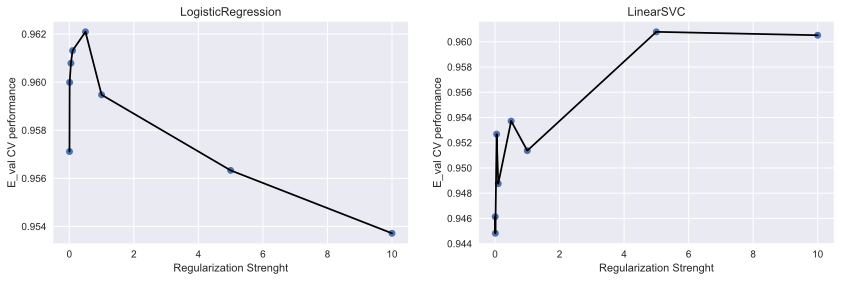
\includegraphics[width=1\textwidth]{figures/fig03}
    \caption{Regularization performance comparison.}
    \end{minipage}}}
\end{figure}

We displayed the performance of the CV tests for adjusting models with both LR and linear-SVM in table 1 and as a comparison of \textit{Acc} in figure 3.

First off, every metric has been displayed up to 3 digit floating point precision but none of them are different until 5 floating point precision, truncating them shouldn't matter to the eyes of our reader, it is clear that these different metrics don't give us distinctive information. 

Second important point, we can see that the Linear-SVM performs worse in the CV tests than the Logistic Regression model.

Thus we took the best performing regularization ($\lambda$) an decided to fix our final hypothesis as $g=\{LogisticRegression, \lambda=5\}$

\subsection{Performance metrics}
Unfortunately this being a multiclass problem the ROC curve becomes a less useful metric due to having to compare multiple graphs, one for each class vs the rest, for every classifier tested.

We opted for evaluating our performance with the \textit{Accuracy} (Acc), \textit{Sensitivity} (Sen) and \textit{Specificity} (Spe) of each model. Sensitivity refers to the rate of correctly classified examples. Specificity refers to the rate of negative examples correctly classified. Accuracy is the total number of correctly classified data divided by the number of examples. This metrics are inspired by the works of \cite{mesejo:hal-01291797} in a recent ML study.

\subsection{Out of sample error}
As in any machine learning problem, our most important goal is a good out of sample error. In this section we will make use of the previously stored fresh (never seen in our training) data points test set in order to estimate the generalization strength of our model.

\begin{minted}{python}
# Path to CSV test data file
filepath_test = 'data/optdigits.tes'
# Create numpy arrays with the data
X_test = genfromtxt(filepath_test, delimiter=',')
y_test = X_test[:,-1]
X_test = X_test[:,0:-1]

# Training final model
final_model = LogisticRegression(tol=1e-5, C=(1/5))
final_model.fit(X_train, y_train)
final_model.score(X_train, y_train)
# Testing the Eout
y_pred = final_model.predict(X_test)
acc = final_model.score(X_test, y_test)

print("Eout: %.3f (1-Accuracity)" % (1-acc))
\end{minted}

\begin{minted}{python}
>>> Eout: 0.052 (1-Accuracity)
\end{minted}

We have to point out that data preprocessing with PCA has been discarded as it hit performance in the tests by a terrible amount $>60 \%$

\subsection{Classification Conclusions}
% Discutir y justificar la calidad del modelo encontrado y las razones por las que considera que dicho modelo es un buen ajuste que representa adecuadamente los datos muéstrales.

\begin{figure}[H]
    \centering
    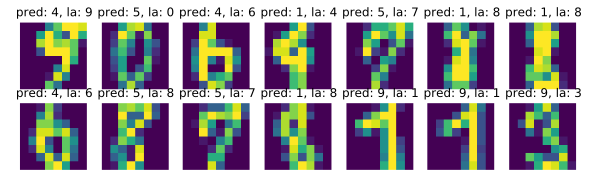
\includegraphics[width=300px]{figures/fig04}
    \label{fig:Dataset visualization}
    \caption{Random subset of mismatched labels}
\end{figure}

To illustrate the empirical results of our classifier we showed multiple numbers from the tests set, titled with the prediction from our final model and the actual label.


We see our tightly dependant to the pixels model falls short when digits like one get slightly shifted to the right, getting confused with nines in our opinion simply because of the placement.

Seeing this results we think there is definitely a big amount of room for improvement, even if a small subset of the digits, like the top-right corner for example, would have a high error rate in human classification in most of the digits displayed a better classifier could definitely have been selected.


\newpage

% \begin{multicols}{2}

{\section{Linear Regression: Airfoil Self-Noise Dataset}}


\subsection{Understanding the problem}
For our second problem we want to make predictions on the sound pressure levels in dB when the wind hits air blades.

To this objective will take a look at the \textit{Airfoil Self-Noise Data Set}. As the previous dataset this data is free and publicly available in the UCI website. \cite{Dua:2019}

As the data set description states: \textit{This data has been obtained through a series of aerodynamic and acoustic tests of two and three-dimensional airfoil blade sections conducted in an anechoic wind tunnel.}

Six attributed where measured in the dataset experiments: Frequency (Hz), Angle of attack (degrees), Chord length (meters), Free-stream velocity (meters per second) and suction side displacement thickness (meters).

Being able to reduce the noise output off air planes by making predictions on how this variables affect the noise would have direct applications for reducing the noise pollution of the air traffic.

With respect to the data set we have a total number of 1503 measurements of these variables in the wind tunnel changing one or multiple variables. Before taking a look at the data we will store a subset for validating our model after fixing our hypothesis:

\begin{minted}{python}
 # Path to CSV training data file
 filepath = 'data/airfoil_self_noise.dat'

 # Load everything
 X = genfromtxt(filepath, delimiter='\t')
 # Take the last column as our label data.
 y = X[:,-1]
 # Remove the column from the set of other characteristics
 X = X[:,0:-1]

 # Split the data in train and test
 X_train, X_test, y_train, y_test = train_test_split(X, y, test_size=0.20)
\end{minted}


\begin{figure}[H]
    \centering
    \makebox[\textwidth]{\makebox[1.35\textwidth]{%
    \begin{minipage}{1.3\textwidth}
        \centering
        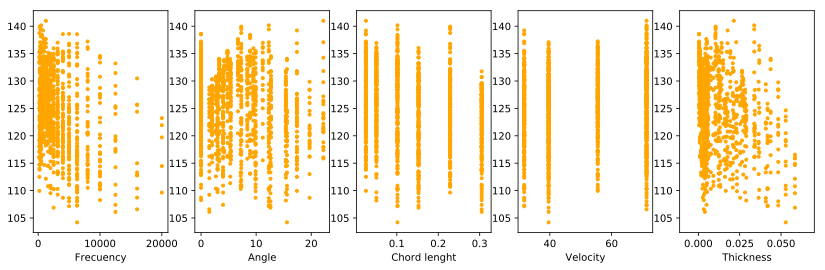
\includegraphics[width=1\textwidth]{figures/r1}
        \caption{Visualisation of every column related to our target (y)}
    \end{minipage}}}
\end{figure}

Now we can take a look at our training split. Plotting every other measured characteristic in relation with our target doesn't reveal much information, there are not apparent relations easily visible to our eye.


\subsection{Data preprocessing} 
As we described in \S2.1, the data set was divided in a 80/20\% split for training and testing respectively.

As the values on the characteristics of the input data come in different ranges, we will \textit{normalise} the training set. Although we won't process the test data initially we will store the min and max values of the training data normalisation to later on, after our hypothesis has been fixed, apply this range of values to the test set too.

\begin{minted}{python}
def normalise(X):
    for i in range(0, X.shape[1]):
        column = X[:, i]
        min_val = min(column)
        max_val = max(column)

        for j in range(0, X.shape[0]):
            if (max_val - min_val) > 0:
                X[j, i] = (X[j, i] - min_val) / (max_val - min_val)

    return X, min_val, max_val
\end{minted}

Even if we only have five dimensions to our input data, after applying normalisation we will run PCA to get an idea if all of this variables are critical to our target predictions on noise levels.

\begin{minted}{python}
 from sklearn.decomposition import PCA
 X_pca = np.copy(X_train)

 pca = PCA(n_components=0.95)
 X_pca = pca.fit_transform(X_pca) 
 print(X_pca.shape)
 print(pca.explained_variance_ratio_) 
\end{minted}

Output:
\begin{code}
\begin{minted}{python}[bgcolor=codepurple, linenos=False]
>>> (1202, 4)
>>> [0.38172358 0.36972943 0.16828515 0.05374699]
\end{minted}
\end{code}
\indent The PCA analysis reveals that four out of the five variables amount for 97\% of the variance in the data. 
Even after considering this results, for the moment we will discard the PCA reduction of dimensionality due to the dimension of the data set being small, only five variables.

\begin{figure}[t]
    \centering
    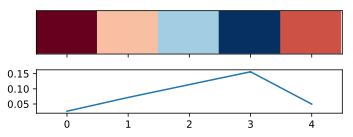
\includegraphics[width=180px]{figures/r2}
    \label{fig:Variance-of-airfoil-data}
    \caption{Heatmap of variance.}
\end{figure}

\subsection{Hypotesis selection}
For selecting our hypothesis we will proceed with a \texit{Structural Risk Minimisation} (SRM) framework in order to get a good fit in our training data minimising the risk of overfitting and being penalised with bad generalisation.

\subsection{Testing methodology}
As in the previous problem discussed in section \S 1 we will use k-folds cross-validation for testing our performance in sample and once our final hypothesis is fixed we will check his generalisation performance with our previously stored validation set (\S 2.1).

\begin{minted}{python}
from sklearn.model_selection import cross_validate
score_metrics = ('neg_mean_squared_error', 'r2') 
rid = linear_model.Ridge(alpha=0.01, copy_X=True) # tol=1e-5,
scores_rid = cross_validate(rid, X_train, y_train, cv=5, 
                                scoring=score_metrics, return_train_score=False)
\end{minted}
\begin{center}
    {\footnotesize Code: Example of testing in sample with sklearn}
\end{center}

\subsection{Regularization}
As discussed in the previous problem \S 1.5 regularization is essential for preventing overfitting and getting a good generalization of our model. To this objective, we will use different regularization strengths in our models testing.

\subsection{Models used and hyperparamethers}
As this is a regression problem where we have to make real values predictions we will fit two extensions of Linear Regression, a Ridge regression (also know as weight decay) model and a Lasso regression model, both are extensions of Linear Regression adding a regularisation factor, we also tested a Support Vector Regression (SVR) model using a linear kernel.


\subsection{Selection and fitting the model}
We performed in sample cross-validation tests with different regularization strengths (Reg), the three lineal models and progressively increasing the hypothesis set($\mathcal{H}$) adding non-linear transformations of our data, polinomials to the power of \textit{'Degree'}.

\begin{table}[H]
\centering
\begin{tabular}{cccccccc}
Classifier & \textit{Degree} & \textit{Reg} & \multicolumn{1}{c|}{MSE} & Classifier & Degree & Reg  & \textit{MSE} \\ \hline
Ridge      & 1               & 0.1          & 23.570                   & Ridge      & 1      & 0.5 & 23.576       \\
Lasso      & 1               & 0.1          & 25.014                   & Lasso      & 1      & 0.5 & 47.840       \\
SVR        & 1               & 0.1          & 23.946                   & SVR        & 1      & 0.5 & 23.624       \\
Ridge      & 2               & 0.1          & 22.269                   & Ridge      & 2      & 0.5 & 22.504       \\
Lasso      & 2               & 0.1          & 25.106                   & Lasso      & 2      & 0.5 & 47.840       \\
SVR        & 2               & 0.1          & 22.816                   & SVR        & 2      & 0.5 & 23.479       \\
Ridge      & 3               & 0.1          & 21.918                   & Ridge      & 3      & 0.5 & 22.264       \\
Lasso      & 3               & 0.1          & 25.121                   & Lasso      & 3      & 0.5 & 47.840       \\
SVR        & 3               & 0.1          & 22.679                   & SVR        & 3      & 0.5 & 23.095       \\
Ridge      & 4               & 0.1          & 21.763                   & Ridge      & 4      & 0.5 & 22.110       \\
Lasso      & 4               & 0.1          & 25.121                   & Lasso      & 4      & 0.5 & 47.840       \\
SVR        & 4               & 0.1          & 22.619                   & SVR        & 4      & 0.5 & 22.859      
\end{tabular}
\end{table}

\begin{table}[H]
\centering
\begin{tabular}{cccccccc}
Classifier & \textit{Degree} & \textit{Reg} & \multicolumn{1}{c|}{MSE} & Classifier & Degree & Reg  & \textit{MSE} \\ \hline
Ridge      & 1               & 0.005        & 23.570                   & Ridge      & 1      & 0.01 & 23.570       \\
Lasso      & 1               & 0.005        & 23.574                   & Lasso      & 1      & 0.01 & 23.585       \\
SVR        & 1               & 0.005        & 24.185                   & SVR        & 1      & 0.01 & 24.178       \\
Ridge      & 2               & 0.005        & 22.261                   & Ridge      & 2      & 0.01 & 22.260       \\
Lasso      & 2               & 0.005        & 22.282                   & Lasso      & 2      & 0.01 & 22.452       \\
SVR        & 2               & 0.005        & 23.301                   & SVR        & 2      & 0.01 & 23.225       \\
Ridge      & 3               & 0.005        & 21.750                   & Ridge      & 3      & 0.01 & \textbf{21.748}       \\
Lasso      & 3               & 0.005        & 22.251                   & Lasso      & 3      & 0.01 & 22.403       \\
SVR        & 3               & 0.005        & 23.339                   & SVR        & 3      & 0.01 & 23.221       \\
Ridge      & 4               & 0.005        & 21.735                   & Ridge      & 4      & 0.01 & 21.724       \\
Lasso      & 4               & 0.005        & 21.994                   & Lasso      & 4      & 0.01 & 22.437       \\
SVR        & 4               & 0.005        & 23.229                   & SVR        & 4      & 0.01 & 23.170      
\end{tabular}
\end{table}

After this results we set our hypothesis as $g=\{Ridge, d_{vc}=15, \lambda=0.01\}$. Although we gained a bit of performance by adding the transformations up to fourth degree, 0.024 MSE, in our opinion this increased fit is not enough to justify the added cost.

\subsection{Performance metrics}
\begin{equation}
    \text{MSE}(y, \hat{y}) = \frac{1}{n_\text{samples}} \sum_{i=0}^{n_\text{samples} - 1} (y_i - \hat{y}_i)^2.
\end{equation}

The metric used for comparing our results is the mean squared error (MSE) as defined by equation 1. This metric has been selected for his simplicity and popularity. It's not a perfect metric by any means because the presence of big outlayers has a great effect on it and could result bad fit but we decided in his use.



\subsection{Out of sample error}
After fixing our final hyphotesis is time to evaluate our results with our test data. We applied the same preprocessing for our test set as our training data and tested our hypothesis with never seen data to finally evaluate the error out of sample.

\begin{minted}{python}
# Processing train data, already normalised
X_train_augmented = augmente_degree(X_train, 3)

# Procesing test data
X_test = normalise_range(X_test, min_training_val, max_training_val)
X_test_augmented = augmente_degree(X_test, 3)

# Training final model
rid = linear_model.Ridge(alpha=0.01, copy_X=True)
rid.fit(X_train_augmented, y_train)

# Testint the Eout
y_pred = rid.predict(X_test_augmented)
mse = mean_squared_error(y_test, y_pred)
\end{minted}

\begin{minted}{python}
>>> Eout: 22.551 MSE
\end{minted}

\subsection{Results}
\begin{figure}[H]
    \centering
    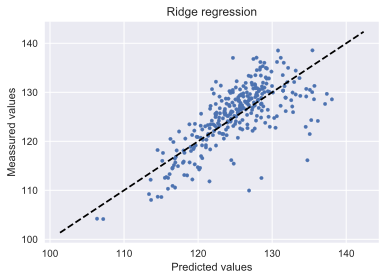
\includegraphics[height=190px]{figures/r3}
    \caption{Comparison predicted vs real values}
    \label{fig:my_label}
\end{figure}

We can say we got very good results within the limitations of the experiment obviously we were limited to lineal models and I'm our opinion they don't seen enough to reflect the complexity of the problem.

We trained a model that generalized decently enough out of sample considering the error in sample wasn't as low as we would have liked it to be.

In figure 7 we can check the relationship between our predictions and the test data split true values. We do observe a tendency and we could say we did learn something.

Through good methodology we obtained a model that can generalize and even if the predictions are not rock solid it can give us a good idea of what the noise levels could be.


\newpage

\bibliographystyle{alpha}
\bibliography{references}

\end{document}
